\chapter{State of the art}
\label{cap2}

In the last years, the drone technology is expanding rapidly;especially the aerial drones, which are often used as toys controlled by joystick  or to make aerial videos through mounted cameras.
There exist also aquatic and terrestrial drones, which can be used for many applications. 
For example, through aquatic drones the submarine network infrastructure\cite{submarine} could be managed more efficiently, and through terrestrial drones some emergency situations, like fires, can be managed without involving human life.

Basically, the mobile sensing through drones represents a technological revolution, opening the way for many applications which could not have been developed with the traditional technologies.
Actually, there are a lot of fields where this new technology could be applied, improving performance and reducing costs:
for example surveillance applications, instructing drones to fly over an area monitoring people, or an application in a domestic context, for example instructing drones to find a lost object or to perform some kind of actions, like bringing some objects to the final user.

In the following section we present three main approaches for programming drones , providing existing examples for each one of them:

\begin{itemize}
\itemsep2pt
\item{
\textit{Drone-level approach}, described in section \ref{droneLevel}
}
\item{
\textit{Swarm-level approach}, described in section \ref{swarmLevel}
}
\item{
\textit{Team-level approach}, described in section \ref{teamlevel}
}
\end{itemize}

The former is focused on the programming of an every single drone, while the second implies basic rules to execute for the whole swarm of drones. The third approach is the most modern work. It creates a middle-ground between drone and swarm approaches, by providing a flexibility in expressing sophisticated collaborative tasks without addressing to a single drone.

After presenting the three main approaches for programming drones, we show some examples of data-flow

\section {Drone-level approach}\label{droneLevel}

In the Drone-level approach, the programmer must manage the single drone, taking care of giving a list of instructions that the drone will perform sequentially.
This approach may be suitable for applications where there is a single drone performing some actions, like searching for a lost object and bringing it back to the user.But scaling the application to a number of drones makes programmer to deal with  concurrency and parallelism. Moreover, battery and crashes/failures should be managed manually for every drone. Finally, timing constraints and a dynamic load balance drastically increase the complexity of the programming. For these reasons drone-level approach is not suitable for a large number of drones.
\\

A concrete example of the application of the Drone-level approach is the so called Robot Create(fig.~\ref{fig:irobot}), a hobbyist robot manufactured by iRobot\cite{irobot} that was introduced in 2007 and based on their Roomba vacuum cleaning platform. The iRobot Create is explicitly designed for robotics development and improves the experience beyond simply hacking the Roomba. 
Since the built-in serial port supports the transmission of sensor data and can receive actuation commands, any embedded computer that supports serial communication can be used as the control system.
\\

To control the Create, the developer should send a sequence of commands through the serial interface. Each command starts with a one-byte opcode and some of them must be followed by data bytes. For example to control the wheel actuators the developer should send a command like this:
\\

\textit{[137] [Velocity high byte] [Velocity low byte] [Radius high byte] [Radius low byte]}
\\

It takes four data bytes, interpreted as two 16-bit signed values using two’s complement. The first two bytes specify the average velocity of the drive wheels in millimeters per second (mm/s), with the high byte being sent first. The next two bytes specify the radius in millimeters at which Create will turn.
\\

\begin{figure}[H]
  \centering
  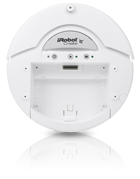
\includegraphics[width=5cm,height=5cm]{pictures/Irobot.png}
  \caption{The iRobot Create}
  \label{fig:irobot}
\end{figure}

A number of robot interface server / simulators support the iRobot Create. Most notably, the Player Project has long included a device interface for the Roomba, and developed a Create interface in Player 2.1. The Universal Real-time Behavior Interface (URBI) environment also contains a Create interface.
This robot is designed for a single execution of a single task without being connected with other robots. Moreover, the design does not imply the collaboration with other robots.
\\

\section{Swarm-level approach}\label{swarmLevel}

The Swarm-level approach\cite{swarm} is more suitable for applications where a number of drones are supposed to perform the same actions. Indeed the programmer can give a set of basic rules that each drone in the swarm can follow.
It is important to underline that, in swarm-level approach, there is no possibility to have a shared state between drones; each drone execute the actions specified by the programmer on his own local state.
It enables the scaling of the approach, but it's not suitable for applications that require the drones to explicitly coordinate.
For example, the swarm-level approach could be applied in an application where many drones take objects at different locations and bring them to the final user, without considering any time or space coordination between them; each drone will simply bring the object back to the user when found.  
There are several existing applications using the swarm-level approach, but we decided to describe three of them:
the Robot Operating System (ROS)\cite{ros}, which provides a Publish/Subscribe coordination layer for decentralized computations, as shown in section \ref{ros}; Karma\cite{karma}, which lets programmers specify modes of operation for the swarm, such as “Monitor” or “Pollinate”(as shown in section \ref{karma}); and Proto\cite{proto}, which lets programmers specify actions in space and time(as shown in section \ref{proto}). 

\subsection{Robot Operating System}\label{ros}

ROS\cite{ros} is not an operating system in the traditional sense, indeed it provides a layer for communication between many, possibly heterogeneous, operating systems connected in a cluster.

The whole functioning of ROS, shown in fig.\ref{fig:ros}, is based on \textit{Nodes}, which are software modules performing computations; the whole system is composed by many nodes exchanging messages, according to the \textit{Publish-Subscribe} model:
a node can send messages publishing them on a particular \textit{Topic}, and nodes which are interested in a particular topic simply subscribe to it; publishers and subscribers don't know each others' existence.
The publish-subscribe topic based communication model is very flexible, but is not suitable for synchronous exchanges, because of its broadcast functioning; for this reasons ROS provides also \textit{Services}, which are composed by a name and two messages, one for the request and one for the response.





\begin{figure}[htbp]
  \centering
  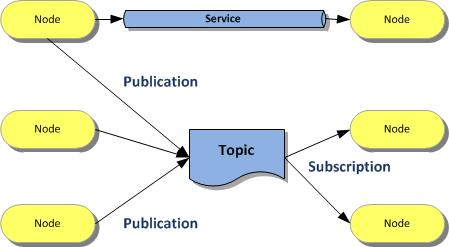
\includegraphics[width=\linewidth]{pictures/ros.jpg}
  \caption{ROS communication layer functioning}
  \label{fig:ros}
\end{figure}


\newpage

\subsection{Karma}\label{karma}

Karma\cite{karma} is a resource management system for drones swarms based on the so called hive-drone model; the hive-drone model is a feature that moves the coordination complexity of the application to a centralized computer: the hive is the base station where drones can land, if they are not busy, and charge their batteries; the hive also takes care of dispatching the drones in order to perform the actions specified by the programmer to accomplish the swarm objectives; the programmer specifies the desired swarm behaviour through a programming model which allows him not to deal with a coordination between drones.

The Karma\cite{karma} runtime at the hive is composed by functional blocks, as shown in fig.~\ref{fig:karma}:

\begin{itemize}
\itemsep2pt
\item{
\textit{Controller}: is the overall manager of the runtime and invokes the other modules when needed; when a user submits an application to the Karma system, the hive Controller determines the set of active processes, and invokes the Scheduler to allocate the available drones to them.
}
\item{
\textit{Scheduler}: is periodically invoked by the Controller to allocate drones to each active process.
}
\item{
\textit{Dispatcher}:  is responsible for tracking the status of the drones; it programs the drones with the allocated behavior prior to a sortie, tracks the size of the swarm, and notifies the Controller when a drone returns to the hive and is ready for redeployment.
}
\item{
\textit{Datastore}: when drones return to the hive, they transfer the data they collected to the Datastore.
}
\end{itemize}


\begin{figure}[htbp]
  \centering
  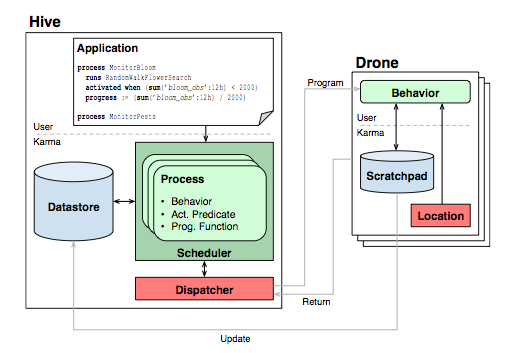
\includegraphics[width=\linewidth]{pictures/Karma.png}
  \caption{The basic schema of Karma}
  \label{fig:karma}
\end{figure}

\newpage

\subsection{Proto}\label{proto}

The amorphous medium abstraction\cite{medium} is derived from the observation that in many spatial computing applications, we are not interested in the particular devices that make up our network, but rather in the space through which they are distributed; indeed, for example, the only things that matter for a sensor network are the values that it senses, not the particular devices it's composed of.
The amorphous medium\cite{medium} takes this concept to the extreme: indeed it is defined as a spatial area with a computational device at every point, as shown in fig.\ref{fig:medium}: Information propagates through this medium at a maximum velocity. Each device is associated with a neighborhood of nearby devices, and knows the "state" of every device in its neighborhood, i.e. the most recent information that can have arrived from its neighbors.



\begin{figure}[H]
  \centering
  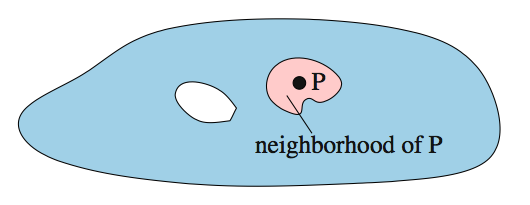
\includegraphics[width=\linewidth]{pictures/ProtoMedium.png}
  \caption{The amorphous medium abstraction}
  \label{fig:medium}
\end{figure}



The Proto\cite{proto} language uses the amorphous medium abstraction\cite{medium} to divide the spatial programming problem in three sub-problems, as shown in fig.~\ref{fig:proto}:

\begin{itemize}
\itemsep2pt
\item{
global descriptions of programs as functional operations on fields of values
}
\item{
compilation from global to local execution on an amorphous medium
}
\item{
discrete approximation of an amorphous medium by a real network
}
\end{itemize}


\begin{figure}[h!]
  \centering
  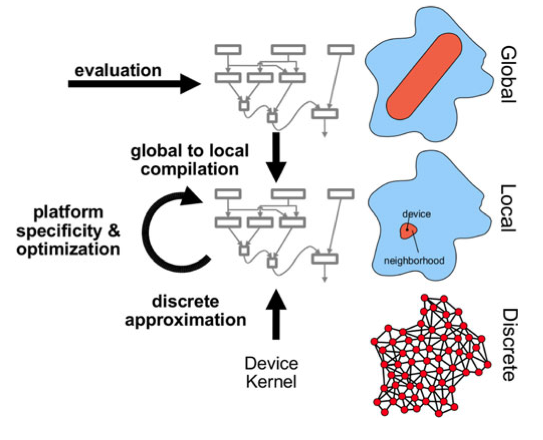
\includegraphics[width=\linewidth]{pictures/Proto.png}
  \caption{Proto: problem decomposition}
  \label{fig:proto}
\end{figure}

To apply Proto\cite{proto} language to mobile devices, such as drones in a swarm, the amorphous medium\cite{medium} must be extended with the concept of \textit{density}; indeed for the vast majority of mobile applications, it is important to distribute drones depending on what is happening in the environment, for example one may want to send more drones in an area where something is happening; so it must be possible to distribute drones heterogeneously in the space.
Adding the concept of \textit{density}, Proto can express a lot of applications using the swarm-level approach.
For example, a swarm of lightweight scout robots might search a disaster area and coordinate with a team of more capable rescue robots that can aid victims, or a swarm of aerial vehicles might team with firefighters to survey and manage wildfires and toxic spills, or a group of autonomous underwater vehicles might survey their environment and autonomously task portions of the swarm to concentrate data gathering on particular interesting phenomena.


\section {Team-level approach}\label{teamlevel}

In this section we describe the team-level programming approach\cite{voltron}, which allows the user to express a list of sensing tasks to be performed by the system, without dealing with the management of the single drone and with complex programming tasks such as concurrent programming and parallel execution; the user can also require a layer of coordination, defining constraints in space and time for the tasks' execution, and the system will follow these constraints choosing the actions for each drone at run-time, in order to collaboratively accomplish all the tasks.
This run-time drones management makes the whole system scalable, since one can add as many drones as he wants, and also fault tolerant, because it can easily manage crashes or exceptions.
So, the main advantage of using the team-level approach is that the user can simply specify a list of tasks to be performed,together with constraints in space and time for the execution, not caring about the dispatching and coordination of the drones; this is also a limitation, because one cannot develop applications which require explicit communication between drones.
So, the team-level approach is most suitable for applications involving tasks that could be also performed by a single drone, but require a large number of drones to be completed faster and/or to operate in a big area.
\\

A concrete example of team-level approach application is Voltron\cite{voltron}, a system containing a set of programming constructs to explore the notion of team-level drone programming. 
Voltron's\cite{voltron} basic functioning includes:

\begin{itemize}
\itemsep2pt
\item{
the so-called \textit{abstract drone}, which makes the application scalable, allowing to add drones without changing the code
}
\item{spatial semantics, which allow the drones to execute parallel tasks at different locations
}
\item{
the possibility to dinamically re-schedule drones operations in case of crashes or failures
}
\item{
the possibility to define time constraints for the tasks 
}
\end{itemize}

Voltron\cite{voltron} exposes an API, as shown in fig.\ref{fig:voltron}, that programmers can use to task the drones without individual addressing; since the abstract drone is the only entry point to the system’s functionality, an application’s code can remain unaltered no matter how many real devices are deployed.
\\

\begin{figure}[htbp]
  \centering
  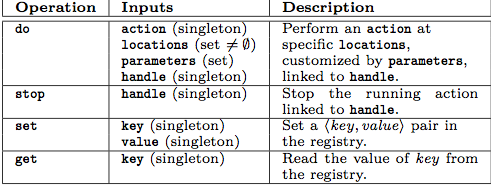
\includegraphics[width=\linewidth]{pictures/Voltron.png}
  \caption{Voltron APIs}
  \label{fig:voltron}
\end{figure}


The team-level approach represents a  middle-ground between the drone-level and swarm-level approaches, and it also solves many problems. Unlike the drone-level approach, there is no need to address the single drone and, unlike the swarm-level approach, there can be a "global state" and also time and space constraints can be defined; as already said, the team-level approach's main limitation is that there is no possibility to perform tasks which require explicit communication between drones, such as passing an object between them.
\\

\section{Data-flow programming}\label{dataflow}

Dataflow Programming is a useful programming paradigm that allows a developer to represent the execution model of his application through a directed graph. The flow of the data processed during the execution streams between all nodes. Each node is a functional block that accept data as input, manages it performing its tasks and then drive it forward to the next block. 
\\
The final dataflow application is nothing but a composition of these active blocks with at least one initial and one ending blocks, connected by directed arrows.
A block is connected to another when it has a dependency on the result of the manipulation of the data from that block. Values are propagated after they are processed from all the dependent blocks triggering their execution.
\\

This paradigm present some limits of expression.
The main one is that each implementation of this paradigm is specific for the context where it is used. This means that there are no general frameworks that can be used in more than one context. This is why we created our own dataflow editor, shown in section \ref{plutoGraphicalEditor}.

\subsection{Business Process Modeling Notation}

Business Process Modeling Notation (BPMN) is an example of the power of the dataflow programming paradigm. Its primary goal is to help business users providing a readily understandable notation, filling the gap between the business process design and the final process implementation.
\\

BPMN defines a diagram that contains graphical models of the business process operations. A Business Process Model, is nothing but a graph where nodes represent graphical models representing the operations, and edges are the flow controls that define their order of performance. An example is shown in figure \ref{fig:bpmn}.
\\

 \begin{figure}[htbp]
   \centering
   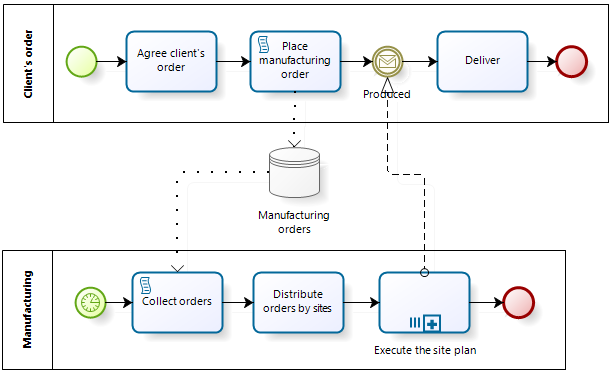
\includegraphics[width=\linewidth]{pictures/bpmn.png}
   \caption{Example of a BPMN diagram}
   \label{fig:bpmn}
 \end{figure}

There are different kinds of elements in a diagram:

\begin{itemize}
\item{\textit{Flow Objects}: they can be Events (circles), Activities (rounded rectangles) or a Gateway (diamonds)}
\item{\textit{Connecting Objects}: they can represent a Sequence Flow (solid line), a Message (dashed line) or an Association (dotted lines)}
\item{\textit{Swimlanes}: they can be a Pool representing the Actor of the process, or a Lane that is a sub-partition within a Pool}
\item{\textit{Artifacts}: they are useful to extend the basic notation adding new ways to describes context based information}
\end{itemize}

\subsection{Node-RED}

Node-RED is an example of the dataflow paradigm applied to the \textit{Internet of Things} world.
It is a browser-based editor that let the developer wire together different nodes with directed edges.
Each node provides a different feature or a different management of the input data.
All features are web-based functionality, such as receiving an HTTP request or a \textit{Javascript} snippet.
In this context, a diagram represents the back-end of the web application and When the graph is completed, the user can deploy it with a single-click in the runtime environment.
\\

The light-weight runtime is built on \textit{Node.js}, taking full advantage of its event-driven, non-blocking model. This makes it ideal to run at the edge of the network on low-cost hardware as well as in the cloud.
\\

In figure \ref{fig:nodeRed} we show an example web application.
\\

 \begin{figure}[htbp]
   \centering
   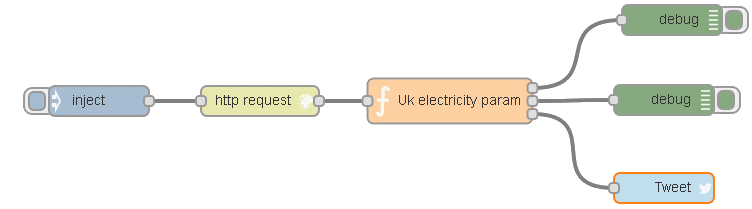
\includegraphics[width=\linewidth]{pictures/nodeRed.png}
   \caption{Example of a nodeRED application}
   \label{fig:nodeRed}
 \end{figure}

The yellow node makes a GET request to the UK electric company website.
\\
The response data follow the edges and pass through the orange node, which lets the developer write its custom Javascript code inside it. 
In this case, the custom code takes the payload data in input and put them on the third output, formatting them in readable way. 
Through the first two outputs, the block sends only debug strings that go to the green nodes.
\\
In the end the blue node will send a tweet containing the data received as input.
\\


\section{Advancement over State of the Art}\label{advancement}

In this chapter we have described the actual state of the art in the field of drone-programming.

We have shown the three main existing approaches for developing drone-based applications and the power of expression of the dataflow programming paradigm.

Since the approaches we mentioned in this chapter are designed in a way that is impossible to describe an application through the concepts of missions and trips, we give our contribution to the state of the art creating a new framework based on these entities.
A \textit{Mission} is nothing but a list of sensing tasks to be performed in the environment.
Each one of these sensing tasks is a \textit{Trip}, that is a movement from a point A to a point B to perform an action.

Neither the drone-level nor the swarm-level approaches are suitable for our goal. 
The former because we do not want the user to deal with the coding of each drone separately with an external API.
The latter because we want to avoid the complexity to create a communication network protocol between drones and because it would be difficult to maintain the status of the missions and trips entities among the swarm. Moreover we also need to address  time and space constraints, which cannot be expressed with this approach.

The most suitable approach for our framework is the team-level model, but we need to apply some modifications to it, in order to make it suitable for our work.
So, we should add the concepts of missions and trips. 
The central brain controls the team of drones according to the mission structure and so according to the sequence of trips contained in it. Executing the trips one by one.
\\

Another very important feature of our work is the transparent dispatching of drones:
the central brain takes care of assigning the drones to the sensing tasks to be performed, managing also the drones failures, without involving the programmer.
\\

Regarding the dataflow programming, we need a new framework that allows the user to design the behavior of the central brain taking care of the missions execution, from the beginning to the end. 
This modeling tool helps the developer to add the features needed by the application simply drawing the proper nodes in the dataflow graph. 
This part of the project is fully described in Section \ref{plutoGraphicalEditor}.



